% Editable native annotations around unchanged verified IDE photographs.
\par
\begin{figure}[htbp]
\centering
\newsavebox{\MARScbordepthregistersBox}
\sbox{\MARScbordepthregistersBox}{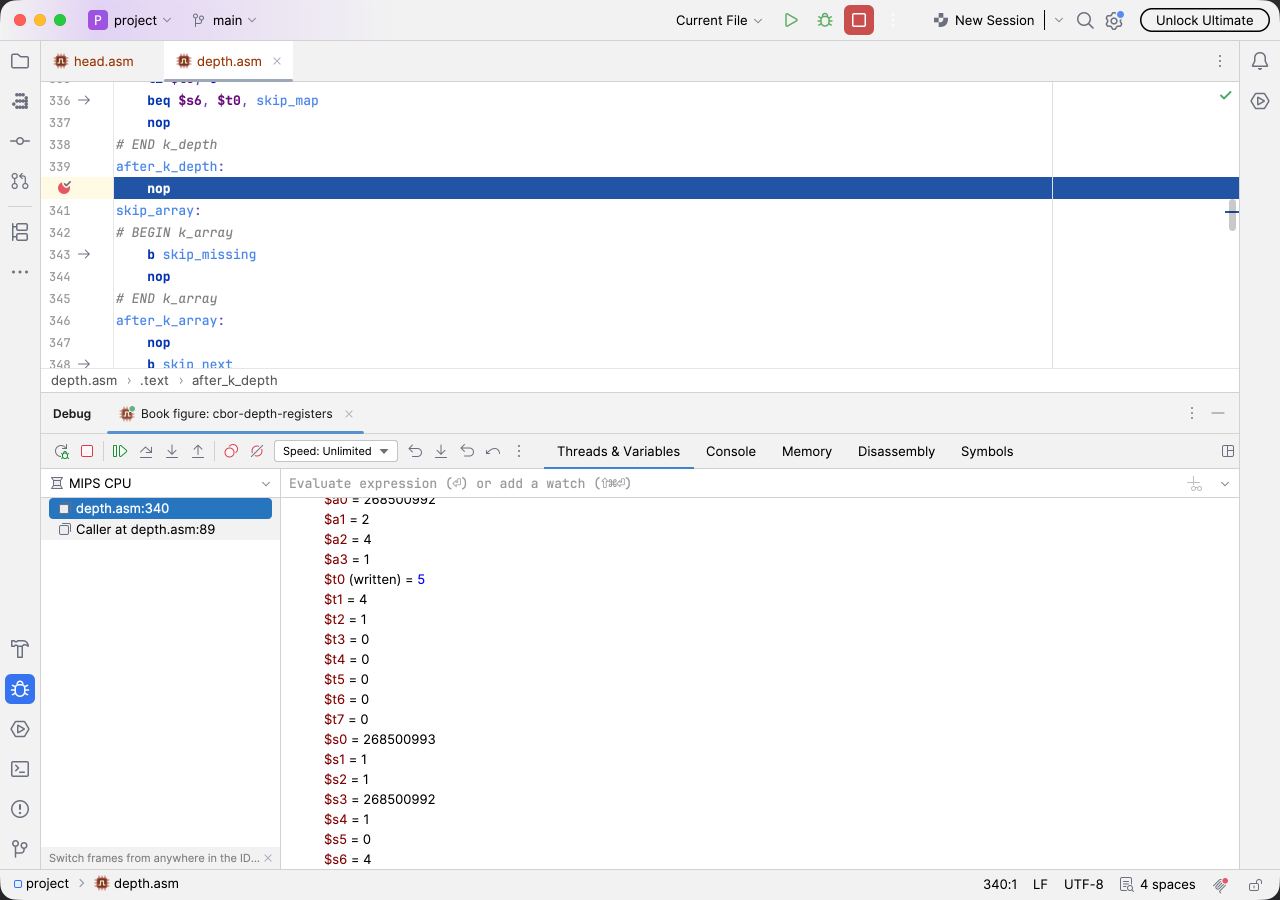
\includegraphics[artifact]{book/captures/032-cbor-telemetry/inherited-depth/registers.png}}
\newsavebox{\MARScbordepthsourceBox}
\sbox{\MARScbordepthsourceBox}{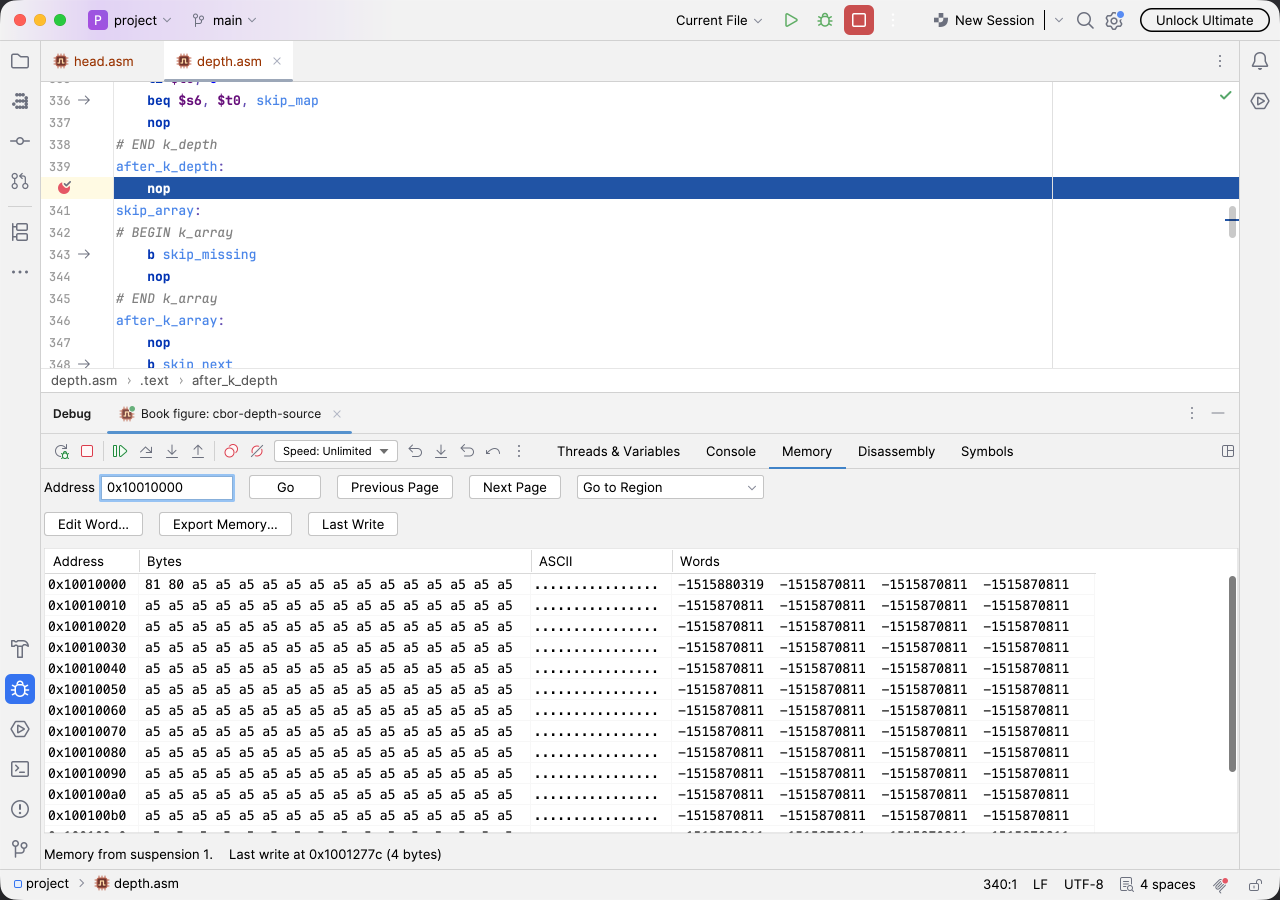
\includegraphics[artifact]{book/captures/032-cbor-telemetry/inherited-depth/source.png}}
\edef\MARScbordepthsourceLeft{\the\dimexpr0.036718750\wd\MARScbordepthregistersBox\relax}
\edef\MARScbordepthsourceBottom{\the\dimexpr0.774444444\ht\MARScbordepthregistersBox\relax}
\edef\MARScbordepthsourceRight{\the\dimexpr0.713281250\wd\MARScbordepthregistersBox\relax}
\edef\MARScbordepthsourceTop{\the\dimexpr0.170000000\ht\MARScbordepthregistersBox\relax}
\edef\MARScbordepthinputLeft{\the\dimexpr0.034375000\wd\MARScbordepthsourceBox\relax}
\edef\MARScbordepthinputBottom{\the\dimexpr0.334444444\ht\MARScbordepthsourceBox\relax}
\edef\MARScbordepthinputRight{\the\dimexpr0.584375000\wd\MARScbordepthsourceBox\relax}
\edef\MARScbordepthinputTop{\the\dimexpr0.608888889\ht\MARScbordepthsourceBox\relax}
\edef\MARScbordepthstateLeft{\the\dimexpr0.246093750\wd\MARScbordepthregistersBox\relax}
\edef\MARScbordepthstateBottom{\the\dimexpr0.122222222\ht\MARScbordepthregistersBox\relax}
\edef\MARScbordepthstateRight{\the\dimexpr0.553906250\wd\MARScbordepthregistersBox\relax}
\edef\MARScbordepthstateTop{\the\dimexpr0.852222222\ht\MARScbordepthregistersBox\relax}
\edef\MARScbordepthcountLeft{\the\dimexpr0.246093750\wd\MARScbordepthregistersBox\relax}
\edef\MARScbordepthcountBottom{\the\dimexpr0.077777778\ht\MARScbordepthregistersBox\relax}
\edef\MARScbordepthcountRight{\the\dimexpr0.553906250\wd\MARScbordepthregistersBox\relax}
\edef\MARScbordepthcountTop{\the\dimexpr0.896666667\ht\MARScbordepthregistersBox\relax}
\begin{tikzpicture}[alt={Four details at after_k_depth show an observation nop, retained depth one in s2 and element count one in s4, and input 81 80 followed by untouched backing bytes.}]
\node[anchor=north west,inner sep=0,font=\small\bfseries] (source-title) at (6mm,0) {Before visiting the next child};
\node[anchor=north west,inner sep=0] (source) at ([yshift=-1mm]source-title.south west) {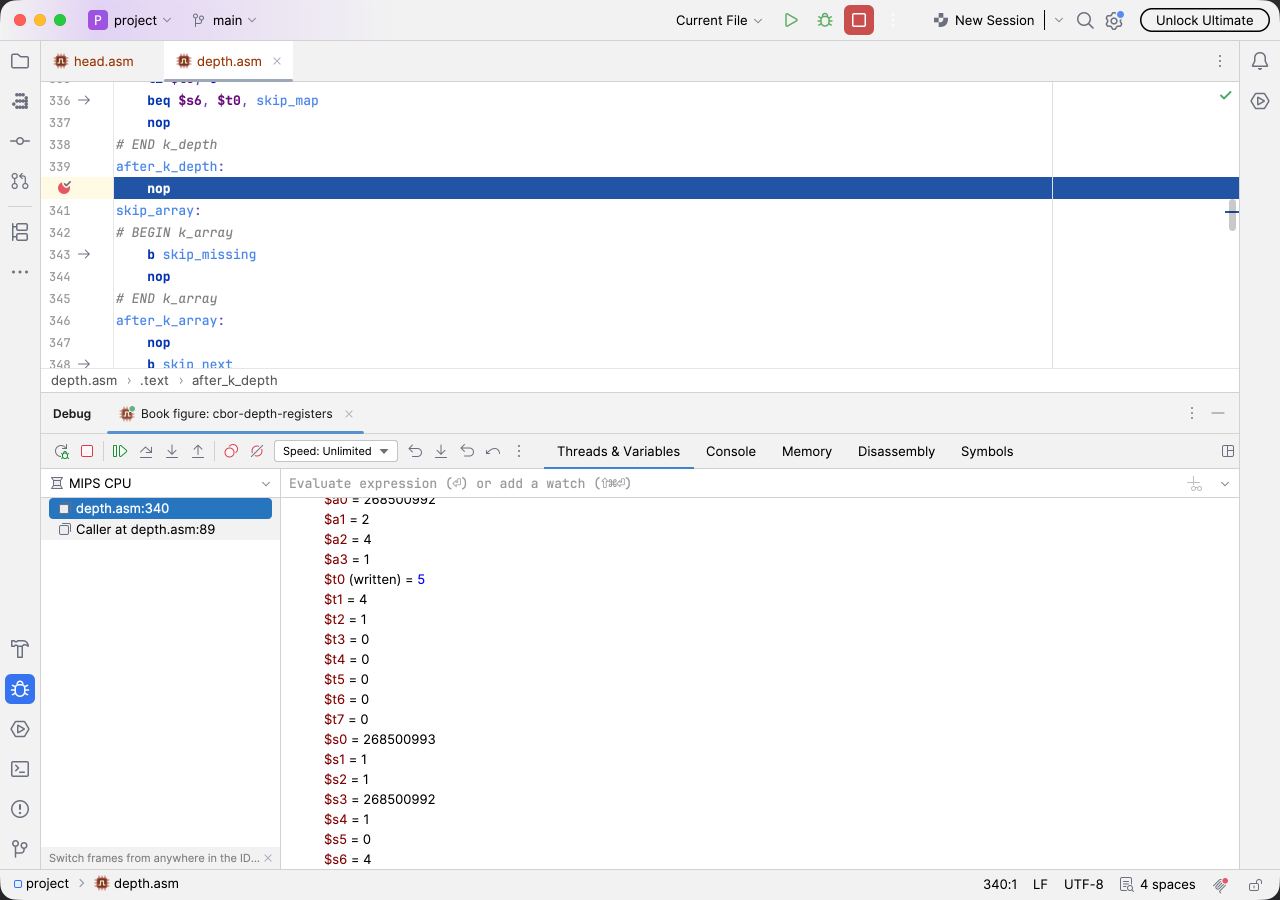
\includegraphics[width=0.54\linewidth,artifact,trim={\MARScbordepthsourceLeft{} \MARScbordepthsourceBottom{} \MARScbordepthsourceRight{} \MARScbordepthsourceTop{}},clip]{book/captures/032-cbor-telemetry/inherited-depth/registers.png}};
\begin{scope}[shift={(source.south west)},x={($(source.south east)-(source.south west)$)},y={($(source.north west)-(source.south west)$)}]
\draw[black,line width=0.7pt] (0.215625000,0.080000000) rectangle (0.384375000,0.520000000);
\node[draw=black,fill=white,circle,inner sep=1.5pt,font=\footnotesize] at ($(0.215625000,0.520000000)+(-3mm,0)$) {1};
\end{scope}
\node[anchor=north west,inner sep=0,font=\small\bfseries] (state-title) at ([yshift=-1mm]source.south west) {Retained open-container depth};
\node[anchor=north west,inner sep=0] (state) at ([yshift=-1mm]state-title.south west) {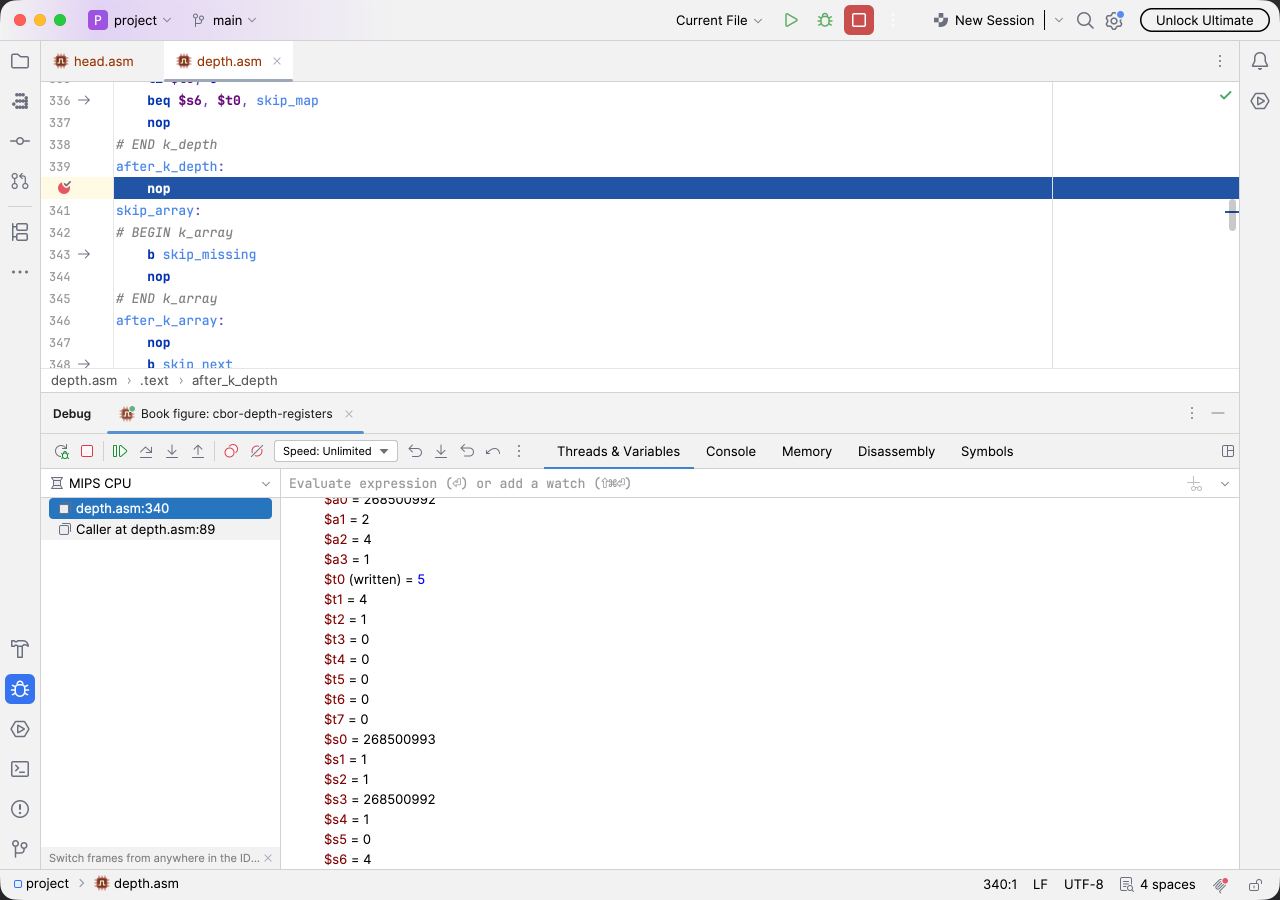
\includegraphics[width=0.48\linewidth,artifact,trim={\MARScbordepthstateLeft{} \MARScbordepthstateBottom{} \MARScbordepthstateRight{} \MARScbordepthstateTop{}},clip]{book/captures/032-cbor-telemetry/inherited-depth/registers.png}};
\begin{scope}[shift={(state.south west)},x={($(state.south east)-(state.south west)$)},y={($(state.north west)-(state.south west)$)}]
\draw[black,line width=0.7pt] (0.023437500,0.043478261) rectangle (0.214843750,0.913043478);
\node[draw=black,fill=white,circle,inner sep=1.5pt,font=\footnotesize] at ($(0.023437500,0.913043478)+(-3mm,0)$) {2};
\end{scope}
\node[anchor=north west,inner sep=0,font=\small\bfseries] (count-title) at ([yshift=-1mm]state.south west) {Child element count};
\node[anchor=north west,inner sep=0] (count) at ([yshift=-1mm]count-title.south west) {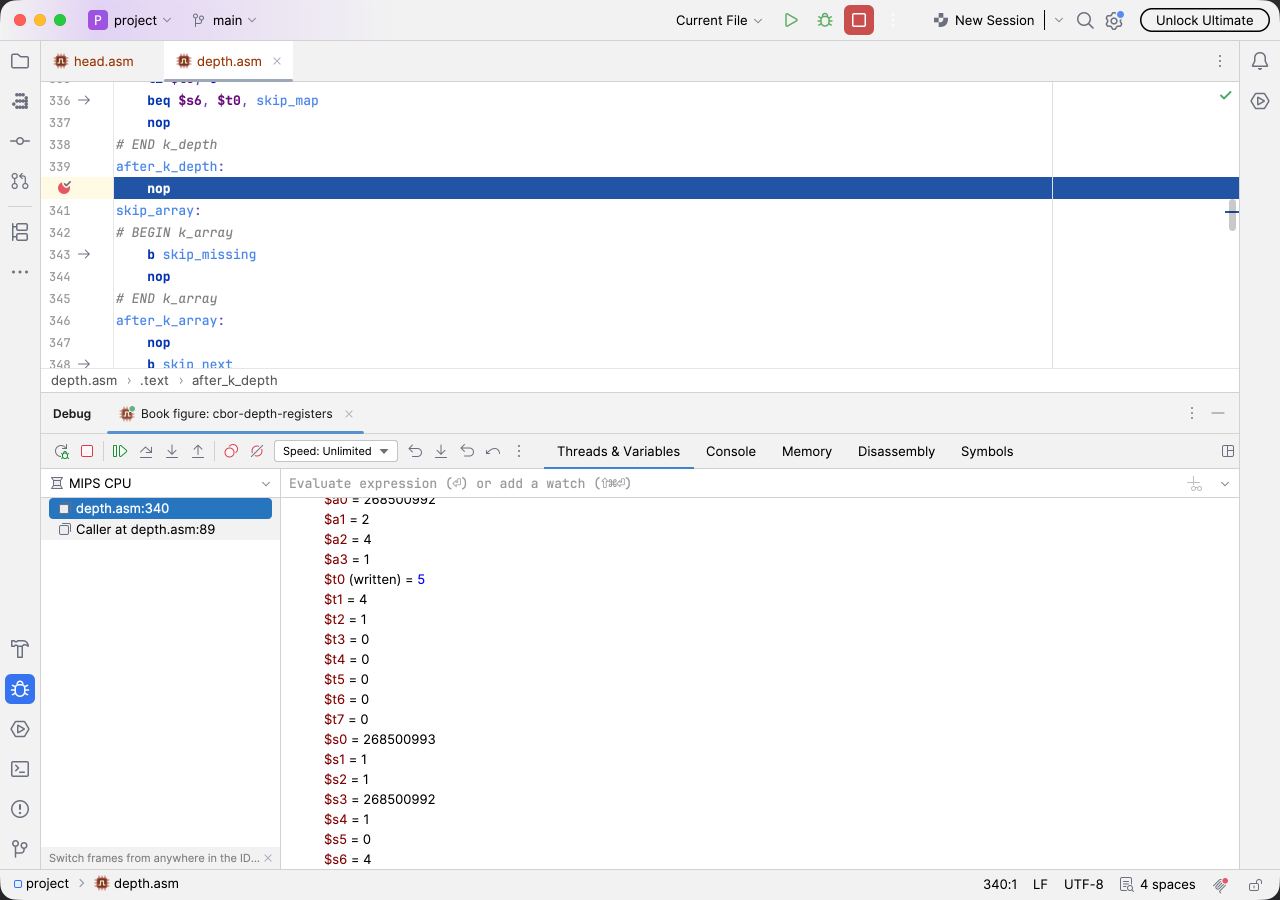
\includegraphics[width=0.48\linewidth,artifact,trim={\MARScbordepthcountLeft{} \MARScbordepthcountBottom{} \MARScbordepthcountRight{} \MARScbordepthcountTop{}},clip]{book/captures/032-cbor-telemetry/inherited-depth/registers.png}};
\begin{scope}[shift={(count.south west)},x={($(count.south east)-(count.south west)$)},y={($(count.north west)-(count.south west)$)}]
\draw[black,line width=0.7pt] (0.023437500,0.043478261) rectangle (0.218750000,0.913043478);
\node[draw=black,fill=white,circle,inner sep=1.5pt,font=\footnotesize] at ($(0.023437500,0.913043478)+(-3mm,0)$) {3};
\end{scope}
\node[anchor=north west,inner sep=0,font=\small\bfseries] (input-title) at ([yshift=-1mm]count.south west) {Outer array and empty child};
\node[anchor=north west,inner sep=0] (input) at ([yshift=-1mm]input-title.south west) {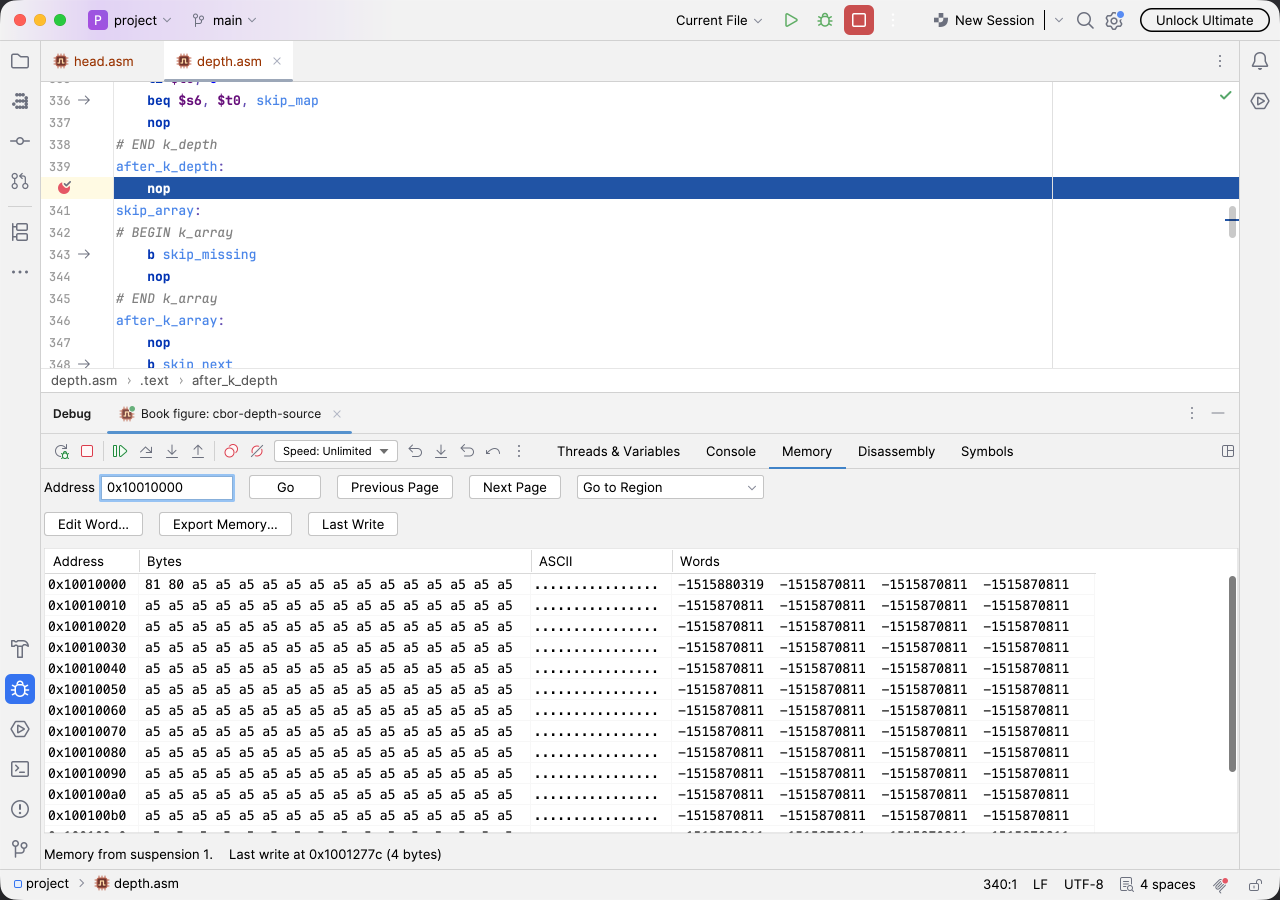
\includegraphics[width=0.84\linewidth,artifact,trim={\MARScbordepthinputLeft{} \MARScbordepthinputBottom{} \MARScbordepthinputRight{} \MARScbordepthinputTop{}},clip]{book/captures/032-cbor-telemetry/inherited-depth/source.png}};
\begin{scope}[shift={(input.south west)},x={($(input.south east)-(input.south west)$)},y={($(input.north west)-(input.south west)$)}]
\draw[black,line width=0.7pt] (0.194672131,0.078431373) rectangle (0.997950820,0.490196078);
\node[draw=black,fill=white,circle,inner sep=1.5pt,font=\footnotesize] at ($(0,0.490196078)+(-3mm,0)$) {4};
\end{scope}
\end{tikzpicture}
\par\smallskip
\begin{minipage}{\linewidth}
\small
\begin{enumerate}
\setlength{\itemsep}{0pt}
\setlength{\parsep}{0pt}
\item The stop follows the depth guard and increment. The caller supplied inherited depth zero; opening this outer container raises the retained count to one. No child has been visited at this checkpoint.
\item \texttt{s2 = 1} records the open outer array. A recursive child must inherit this depth; restarting it at zero would defeat the nesting limit.
\item \texttt{s4 = 1} is the outer array\textquotesingle s element count. It bounds that array\textquotesingle s iteration, independently of the number of open containers.
\item \texttt{81 80} encodes a one-element array containing an empty array. The \texttt{a5} bytes are backing storage beyond the selected two-byte input. An empty array still opens a container. The later child-walk region is unfinished in this cumulative stage, so continuing returns development status four; this image is not evidence of completed recursion.
\end{enumerate}
\end{minipage}
\caption{The walker retains its open-container depth before visiting a child.}
\label{capture:032-cbor-telemetry-inherited-depth}
\label{cbor-inherited-depth}
\end{figure}
\par
